\chapter{Validierung} \label{Validierung}

%%%%%%%%%%%%%%%%%%%%%%%%%%%%%%%%%%%%%%%%%%%%%%%%%%%%%%%%%%%%%%%%
% Überblick
%%%%%%%%%%%%%%%%%%%%%%%%%%%%%%%%%%%%%%%%%%%%%%%%%%%%%%%%%%%%%%%%

\section{Überblick} \label{ValidUeberblick}
Ziel der Validierungsphase ist das Testen auf dem fertigen Board, anhand von Testpersonen. Der Weg bis dahin muss aber ebenfalls controlliert und geprüft sein. Zur Sicherstellung der Funktionalität werden die Komponenten einzeln als auch gesamthaft getestet. 
Jeder Hardware-Bestandteil – Brett, Steuerung, Stromversorgung und Motoransteuerung - hat also sein eigenes Testkonzept.

%%%%%%%%%%%%%%%%%%%%%%%%%%%%%%%%%%%%%%%%%%%%%%%%%%%%%%%%%%%%%%%%
% Brett
%%%%%%%%%%%%%%%%%%%%%%%%%%%%%%%%%%%%%%%%%%%%%%%%%%%%%%%%%%%%%%%%
\section{Brett} \label{ValidBrett}
Das Brett selber, die gepressten Birkenholzplatten, dessen Bearbeitung und die darauf befindliche Stromleiter und Gehäuse wurden einem Stabilitätstest unterzogen, wo geprüft wurde, ob die Komponenten ein Ausreizen der Flexibilität des Brettes vertragen. Die Verbindungen wurden durchgemessen. Es wurde keine Widerstandserhöhung festgestellt. Das Brett selber ist auch nicht zerbrochen.

%%%%%%%%%%%%%%%%%%%%%%%%%%%%%%%%%%%%%%%%%%%%%%%%%%%%%%%%%%%%%%%%
% Magic Glove
%%%%%%%%%%%%%%%%%%%%%%%%%%%%%%%%%%%%%%%%%%%%%%%%%%%%%%%%%%%%%%%%
\section{Steuerung - Magic Glove} \label{ValidSteuerMagicGlove}
Für die Validierung des Magic Glove wurde eine Hand 3D-gedruckt und ein seperater Empfänger mit einem Arduino gebaut, welcher die empfangenen Daten über eine serielle Verbindung an einen Computer sendet. Die Hand wird nun von Minima zu Maxima gebeugt und die gemessenen Werte aufgezeichnet. Somit kann garantiert werden, dass der maximale Bewegungsradius aufgelöst wird und die Daten korrekt gesendet werden.
\begin{figure} [H]
	\centering
	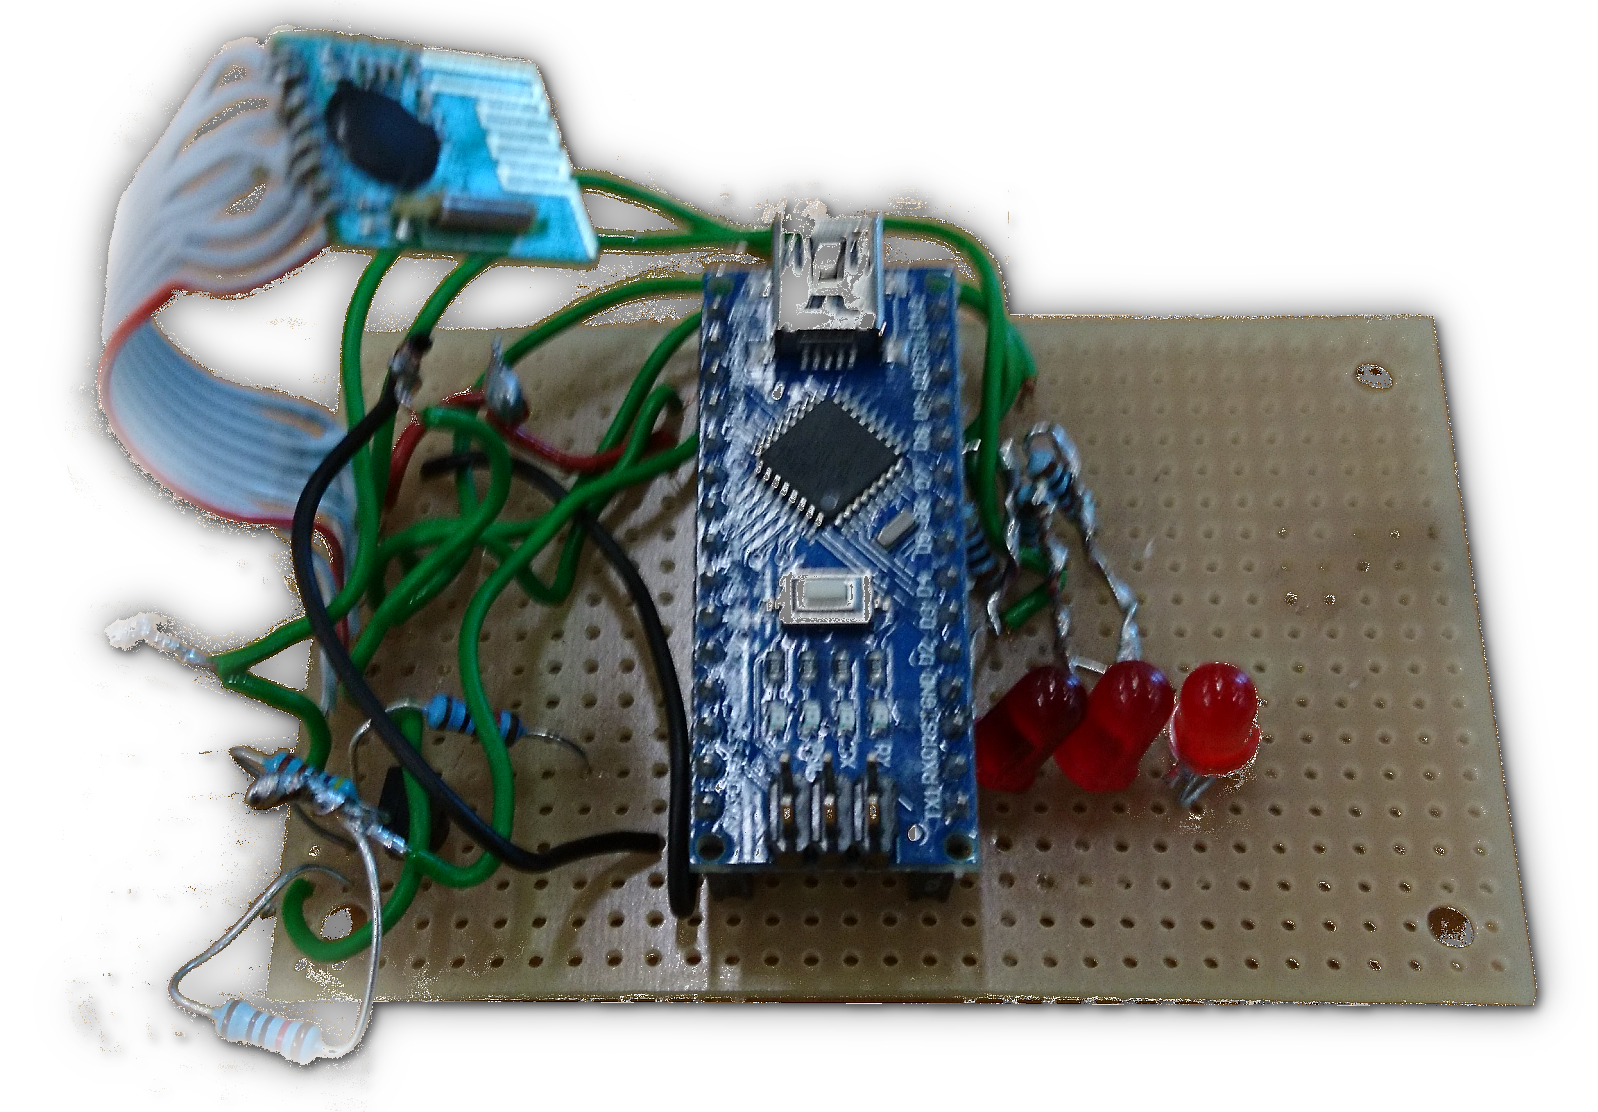
\includegraphics[scale=0.2]{images/receiver}
	\caption{Empfänger zur Validierung des Magic Glove}
	\label{fig:statediagrammbatteri}
\end{figure}
%%%%%%%%%%%%%%%%%%%%%%%%%%%%%%%%%%%%%%%%%%%%%%%%%%%%%%%%%%%%%%%%
% Stromversorgung
%%%%%%%%%%%%%%%%%%%%%%%%%%%%%%%%%%%%%%%%%%%%%%%%%%%%%%%%%%%%%%%%
\section{Stromversorgung} \label{ValidStromversorgung}

%%%%%%%%%%%%%%%%%%%%%%%%%%%%%%%%%%%%%%%%%%%%%%%%%%%%%%%%%%%%%%%%
% MC
Damit die Ergebnisse reproduzierbar sind, wird die Stromversorgung auf einem Prüfstand getestet. In der ersten Validierungsphase wird der Print und die Software ohne Akku getestet, welcher dann in der zweiten Valierungsphase angeschlossen wird. \textbf{Achtung:} Da es sich beim Akku um einen Lithium-Polymer Akku handelt, welcher einen Spitzenstrom von bis zu 500A liefert, sollte der Print zuerst auf allfälligen Kurzschluss geprüft werden.   

\textbf{Hardware}
\begin{itemize}
	\item Funktion der FETs
	\item Messung der Spannungen
	\item Ausmessung des Highside-Driver
\end{itemize}
\textbf{Software}
\begin{itemize}
	\item Einlesen Spannung und Ströme
	\item PWM-Regelung
	\item Balancing Steuerung
\end{itemize}

\subsection*{Hardware}
\subsubsection*{FETs}
Als erstes werde die FETs des Balancing der Reihe nach eingeschaltet. Dabei wird jeweils eine Spannung von 4.2V zwischen Zellanschluss 6 und 5, Zellanschluss 5 und 4 usw. angeschlossen. Sobald die richtige Spannung angeschlossen ist und derjenige FET durchgeschaltet ist, sollte einen Strom von 100mA fliessen. 

\begin{center}
	\begin{tabular}{|c|c|}
		\hline 
		Messobjekt & Strom \\ \hline
		Balance Zelle 1 & $**mA$ \\ \hline
		Balance Zelle 2 & $**mA$ \\ \hline
		Balance Zelle 3 & $**mA$ \\ \hline
		Balance Zelle 4 & $**mA$ \\ \hline
		Balance Zelle 5 & $**mA$ \\ \hline
		Balance Zelle 6 & $**mA$ \\ \hline
	\end{tabular} 
	\captionof{table}{Balancing Strom je Zelle}
	\label{tab:StromBalancing}
\end{center}

Weiter werden die FETs getestet, welche die Spannung zum Motorkontrollboard steuern. Dabei wird einen Leistungswiderstand auf Masse geschaltet. 

\begin{center}
	\begin{tabular}{|c|c|}
		\hline 
		Versorgungsspannung & $25V$ \\ \hline
		Lastwiderstand & $2.5\Omega$ \\ \hline
	\end{tabular} 
	\captionof{table}{Messbedingungen FETs zu Motorcontroll}
	\label{tab:fetmessbedzumotorcontrol}
\end{center}

Nun sollte ein Strom von rund 10A fliessen. Dabei sollten die FETs nur leicht bzw. gar nicht warm werden.

\begin{center}
	\begin{tabular}{|c|c|}
		\hline 
		Strom & $***A$ \\ \hline
	\end{tabular} 
	\captionof{table}{Strom durch Motorcontrol-FET}
	\label{tab:StromMotorcontrollFET}
\end{center}

Der FET welcher fürs Laden zuständig ist, wird bei der Ausmessung des Highside-Driver getestet.

\subsubsection*{Spannungsmessung}
Nun werden die einzelnen Spannungsteiler ausgemessen. Dabei wird am Balancing Anschluss die einzelnen Zellen angeschlossen. Weiter wird die Ladespannung angeschlossen. Nun sollte an den Spannungsteiler gemessen werden. Der Akku sollte voll geladen sein und die Spannungsteiler dürfen die Microcontrollerspeissung nicht überschreiten.

\begin{center}
	\begin{tabular}{|c|c|}
		\hline 
		Versorgungsspannung Batterieseitig & $25V$ \\ \hline
		Versorgungsspannung Ladeseitig & $30V$ \\ \hline
		Versorgungsspannung Mikrokontroller & $5V$ \\ \hline
		Versorgungsspannung Highside-Driver & $15V$ \\ \hline
		
	\end{tabular} 
	\captionof{table}{Messbedinung Spannungsmessungen}
	\label{tab:BedingungSpannungsmessungen}
\end{center}

Um zu Prüfen, ob die Spannungsregelung funktioniert, wurde auch diese gemessen.

\begin{center}
	\begin{tabular}{|l|c|c|}
		\hline 
		Messobjekt & Gemessene Spannung & Skalierungsfaktor \\ \hline
		Versorgungsspannung Mikrokontroller & $5.016V$ & - \\ \hline
		Versorgungsspannung Highside-Driver & $15.65V$ & - \\ \hline
		Zelle 1 & $4.132V / 4.132V$ & 1 \\ \hline
		Zelle 2 & $8.268V / 4.077V$ & 0.493 \\ \hline
		Zelle 3 & $12.34V / 4.064V$ & 0.329 \\ \hline
		Zelle 4 & $16.45V / 4.096V$ & 0.249 \\ \hline
		Zelle 5 & $20.85V / 4.153V$ & 0.202 \\ \hline
		Zelle 6 & $24.72V / 4.120V$ & 0.162 \\ \hline
		Spannungsteiler Ladeseitig & $30.01V / 2.132V$ & 0.071\\ \hline
	\end{tabular} 
	\captionof{table}{Gemessene Spannung}
	\label{tab:Spannungsmessungen}
\end{center}

Die Skalierungsfaktoren lagen ziemlich genau an unserem gewünschten Ergebnis. Somit konnten die berechneten Werte für die Widerstände übernommen werden.  

\subsubsection*{Highside-Driver}
\label{Highside-Driver}
Damit der Highside-Driver getestet werden kann, sollte die Batterie entfernt und einen Leistungswiderstand von rund 5$\Omega$ angeschlossen werden. Der Highside-Driver wird dabei extern mit 15V gespiesen. Als erstes wird am Mikrocontroller ein PWM mit 50\% Duty-Cycle ausgegeben. Dabei sollte am Ausgang des Highside-Driver dasselbe Signal mit 15V Spannungsspitze anliegen. Nun wird eine externe Ladespannung angeschlossen. Diese liegt für Testzwecke bei 15V. Dabei sollte die Strombegrenzung auf 3A eingestellt sein. Nun wird der Duty-Cycle ständig erhöht. Dabei wird der Strom beim Leistungswiderstand gemessen und mit nachfolgender Tabelle abgeglichen.

\begin{center}
	\begin{tabular}{|c|c|}
		\hline 
		Duty-Cycle: 0\% & $0A$ \\ \hline
		Duty-Cycle: 20\% & $0.6A$ \\ \hline
		Duty-Cycle: 40\% & $1.2A$ \\ \hline
		Duty-Cycle: 60\% & $1.8A$ \\ \hline
		Duty-Cycle: 80\% & $2.4A$ \\ \hline
	\end{tabular} 
	\captionof{table}{Ladestrom bei verschiedenen Duty-Cycle}
	\label{tab:LadestromHighsideDriver}
\end{center}

Einen Duty-Cycle von 100\% wird nicht geprüft, da der Highside-Driver nicht dazu ausgelegt ist einen FET dauerhaft durch zusteuern.

Dies konnte aufgrund eines defekten Highside-Driver nicht evaluiert werden. \todo{Wenn bis Mittwoch doch möglich, unbedingt Graphik einbinden, dann kann dieser text gelöscht werden}

\subsection*{Software}
Um diese Ergebnisse zu überprüfen, muss am UART des Mikrocontroller ein TTL-Kabel angeschlossen werden.

\subsubsection*{ADC}
Um die einzelnen Zellen auszulesen, kann die Batterie sowie eine Ladespannung von mindestens 30V angeschlossen werden. Dabei werden die einzelnen Spannungen jede Sekunde einmal über den UART Port ausgegeben. Dabei sollte die Spannung mit dem Multimeter gemessen und überprüft werden. Um denn Strom zu messen, wird die Messung gleich wie in Kapitel \ref{Highside-Driver} aufgebaut. 

\begin{center}
	\begin{tabular}{|l|c|c|c|}
		\hline 
		ADC-Eingang & Spannung Flucke & Spannung ADC & Differenz \\ \hline
		Zelle 1 & $4.132V$ & $4.116V$ & $0.016V$ \\ \hline
		Zelle 2 & $4.134V$ & $4.121V$ & $0.013V$ \\ \hline
		Zelle 3 & $4.065V$ & $4.028V$ & $0.037V$ \\ \hline
		Zelle 4 & $4.117V$ & $4.106V$ & $0.011V$ \\ \hline
		Zelle 5 & $4.132V$ & $4.131B$ & $0.001V$ \\ \hline
		Zelle 6 & $4.131V$ & $4.111V$ & $0.020V$ \\ \hline
		Ladespannung & $***$ & $***$ & $***$ \\ \hline
		Strom & $***$ & $***$ & $***$ \\ \hline
	\end{tabular} 
	\captionof{table}{Ladestrom bei verschiedenen Duty-Cycle}
	\label{tab:LadestromHighsideDriver}
\end{center}

All diese Werte liegen innerhalb der Toleranz des ADCs des Mikrocontrollers und sind somit genug genau.

\subsubsection*{PWM-Regelung}
Um zu überprüfen wird Software-Seitig ein vordefinierter Strom eingestellt. Dabei wird anstatt der Akku ein veränderbarer Leistungswiderstand am Ausgang angeschlossen. Nun wird der Widerstand verändert und überprüft, ob die Software richtig nachregelt.
\begin{center}
	\begin{tabular}{|c|c|}
		\hline 
		Teststrom & $1A$ \\ \hline
		${f}_{PWM}$ & $32kH$ \\ \hline
	\end{tabular} 
	\captionof{table}{Ladestrom bei verschiedenen Duty-Cycle}
	\label{tab:LadestromHighsideDriver}
\end{center}

\todo{Hier muss noch ein KO-bild eingefügt werden.} 

\subsubsection{Balancing-Regelung}
Für diese Validierung wird jeweils eine Spannung an den Zellen Anschlüssen angeschlossen. Dabei wird überprüft, ob die Software bei den jeweiligen Zellen die FETs durchsteuert, um  die gleiche Spannung wie bei den anderen Zellen zu erreichen.

\todo{Wie sollte dies bewiesen werden, das es Validiert wurde?}


%\begin{itemize}
%\item Einlesen Spannung und Ströme
%\item PWM-Regelung
%\item Balancing Steuerung
%\end{itemize}

%%%%%%%%%%%%%%%%%%%%%%%%%%%%%%%%%%%%%%%%%%%%%%%%%%%%%%%%%%%%%%%%
\section{Motoransteuerung} \label{ValidMotoransteuerung}
Um reproduzierbare Ergebnisse zu erzielen, wird die Motoransteuerung auf einem Prüfstand getestet. Dazu wird der Motor ohne Last befestigt und die Schaltung von einem Netzteil gespiesen. Weiter wird die Motoransteuerung in einzelnen Blöcken validiert. Dabei wird unterschieden in Hardware und Software.\\
\\
\textbf{Hardware}
\begin{itemize}
	\item Funktion der FETs
	\item Spannungsmessung mit Spannungsteiler
\end{itemize}
\textbf{Software}
\begin{itemize}
	\item Einlesen der Spannungen und Ströme
	\item SVPWM Raumvektormodulation
	\item Positions- und Geschwindigkeitsbeobachter
	\item D und Q Stromregler
\end{itemize}

\subsection*{Hardware}
\subsubsection*{FETs}
Die FETs werden der Reihe nach von der Software eingeschaltet. Zum Test der FETs wird am Ausgang ein Widerstand auf Masse geschaltet. So kann die Spannung am Ausgang gemessen und aufgezeichnet werden. Zusätzlich wird die Gatespannung gemessen.

\begin{center}
	\begin{tabular}{l|c}
		\hline 
		Versorgungsspannung & $15V$ \\ \hline
		Lastwiderstand & $1k\Omega$ \\ \hline
		Gatestrom Treiber & $1.7A$ \\ \hline
	\end{tabular} 
	\captionof{table}{Messbedingungen FETs}
	\label{tab:fetmessbed}
\end{center}

Zur Gunsten der Übersichtlichkeit wird nur die Messung eines FETs dargestellt.

\begin{figure} [H]
	\centering
	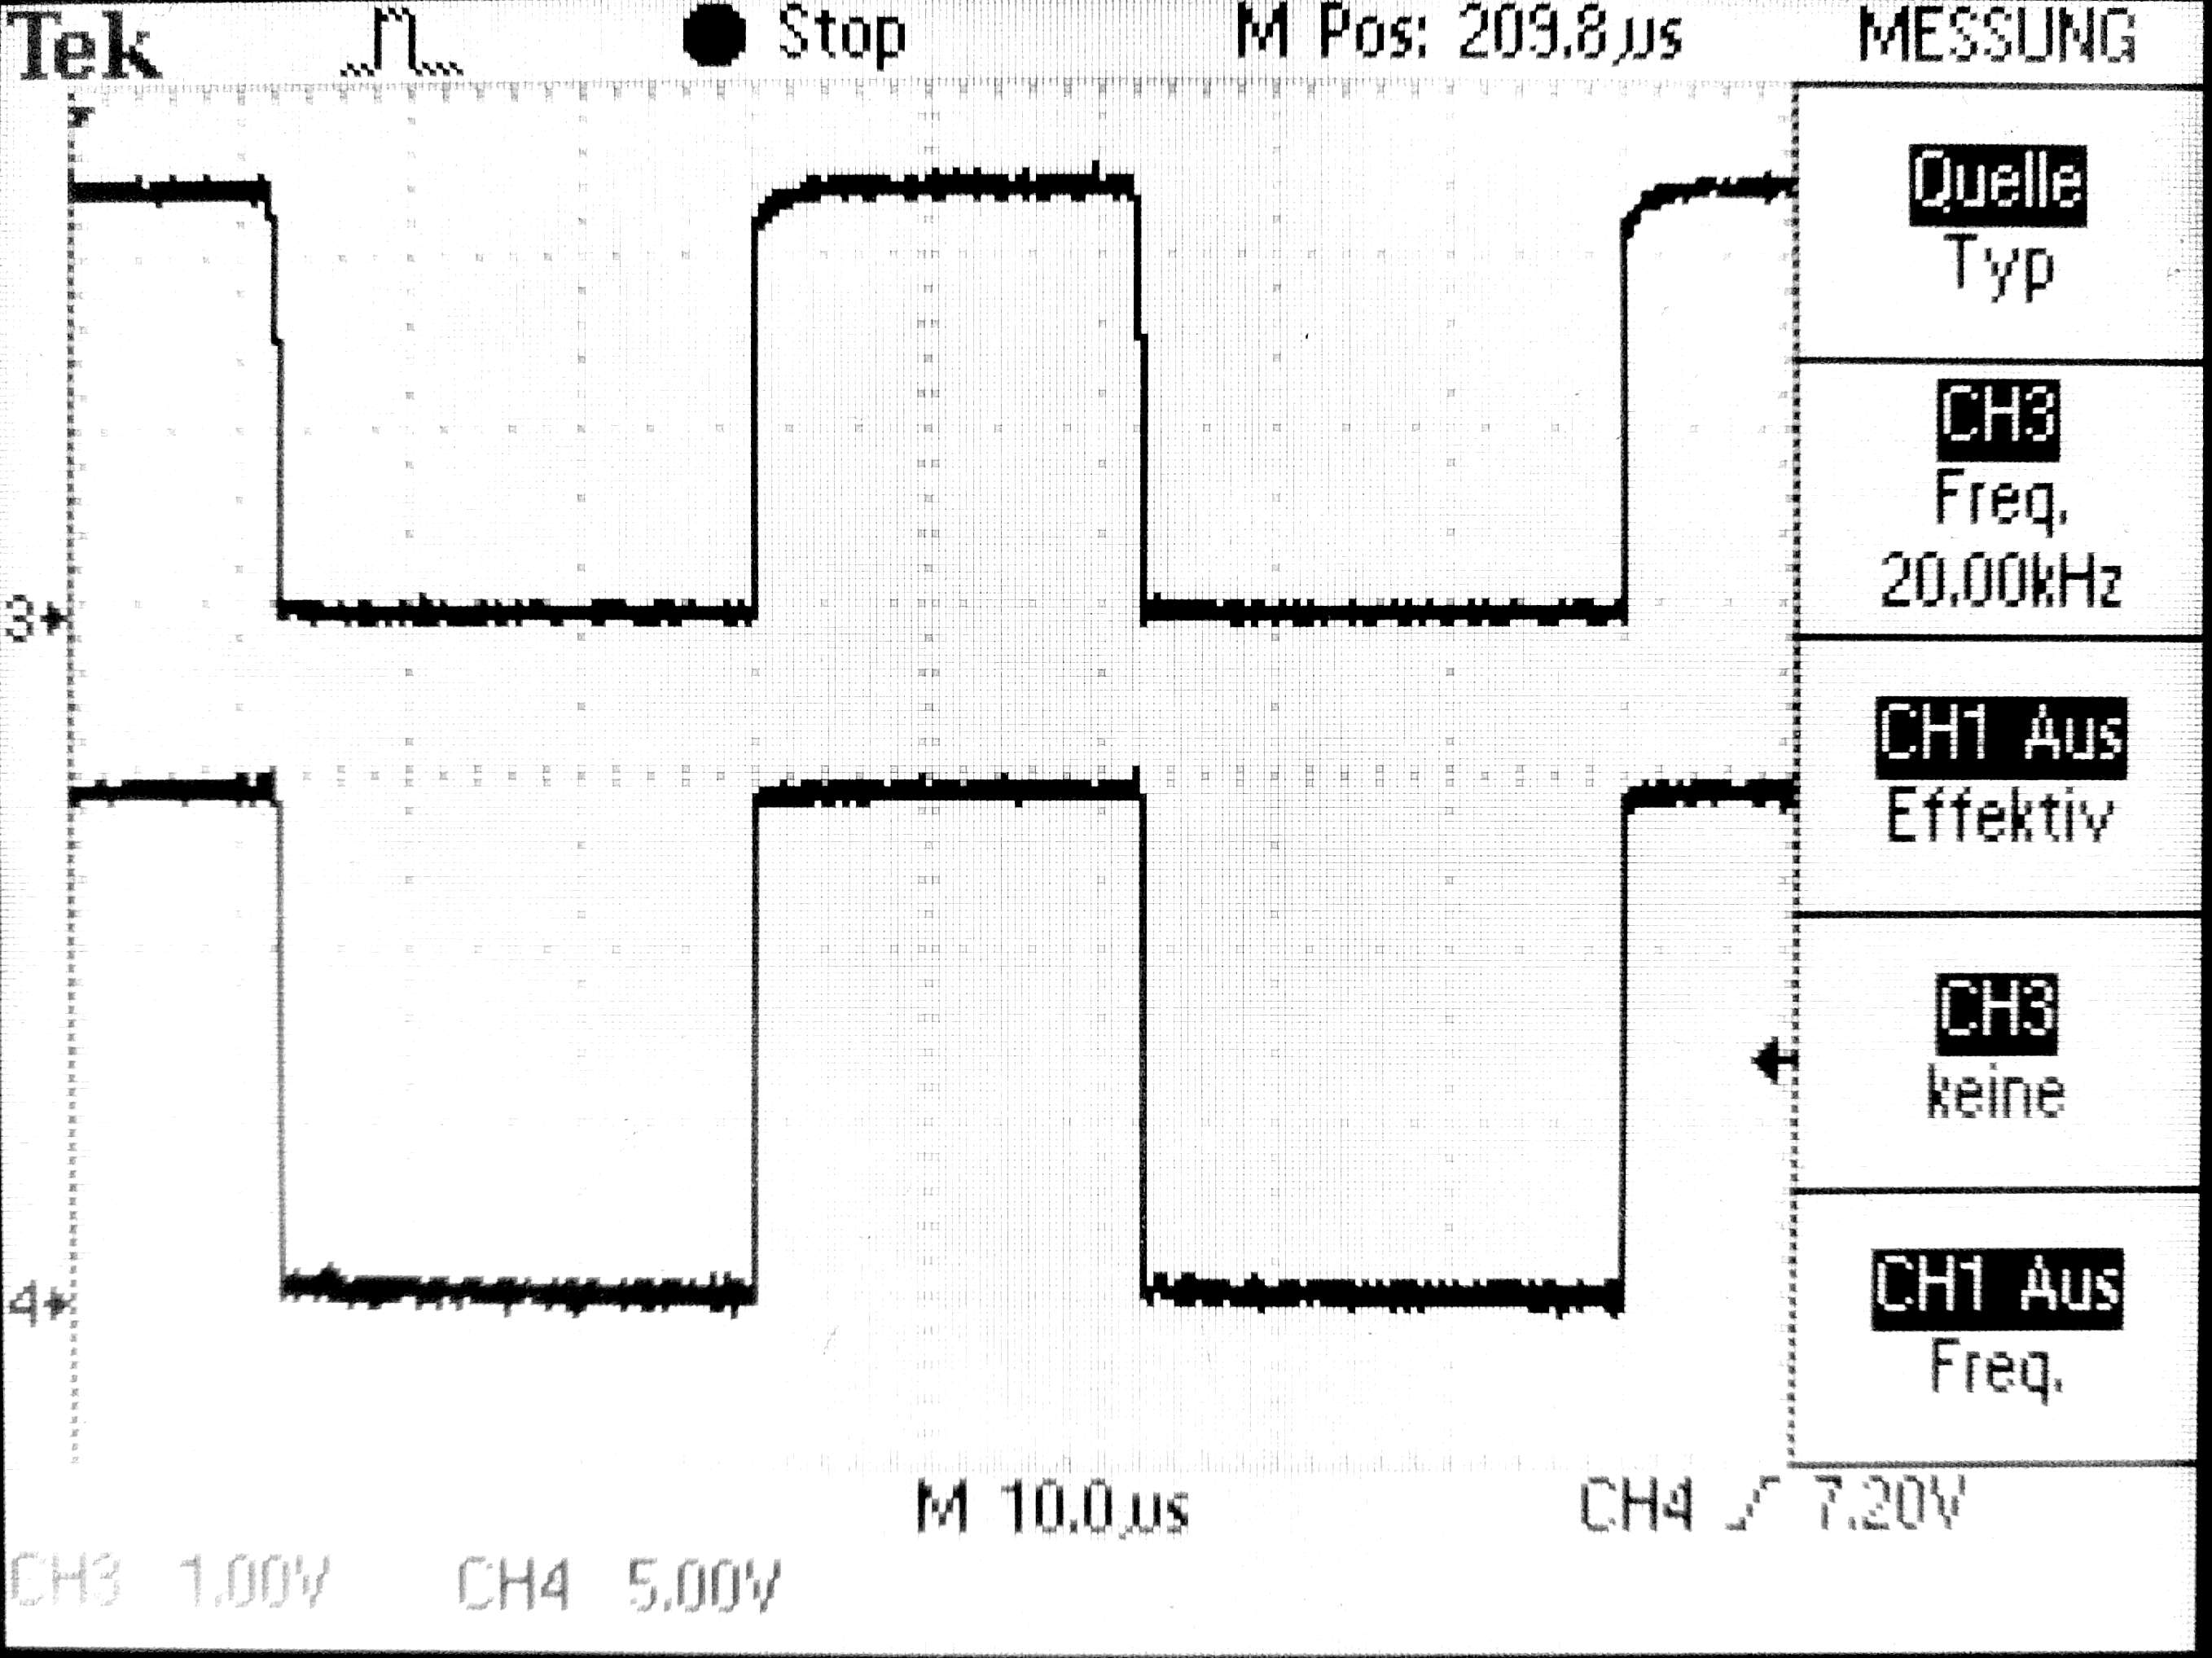
\includegraphics[width=0.5\linewidth]{images/valmcfet.jpg}
	\caption{Einschalten High-Side-FET}
	\label{fig:hsfet}
\end{figure}
\begin{center}
	\begin{tabular}{l|l|l}
		\hline 
		Kanal 1 & High FET A Gate & Mit 10x Abschwächung\\ \hline
		Kanal 2 & Spannung Phase A & {}\\ \hline
	\end{tabular}
	\captionof{table}{Scopeeinstellungen}
\end{center}

Der Kanal 1 zeigt die Steuerspannung am Gate des FETs. Sie wird vom Treiber IC erzeugt und beträgt im eingeschalteten Zustand 24V, das sind rund 7V Gate-Source Spannung. Dies versichert ein schneller Durchschalten des FETs. Erkennbar ist dies an der schnellen Flank am Ausgang der Halbbrücke, zu sehen auf Kanal 4.

\subsubsection*{Spannungsmessung}
Ist der Mikrocontroller im Resetzustand, sind alle FETs ausgeschaltet. So kann eine Spannung an die Ausgänge der H-Brücke gegeben und am Ausgang der Spannungsteiler die Spannung gemessen werden. Diese darf bei einem bestimmten Eingangsspannungsbereich die Mikrocontrollerspeisung nicht überschreiten.

\begin{center}
	\begin{tabular}{l|c}
		\hline 
		Versorgungsspannungsbereich & $0$ bis $20V$ \\ \hline
		Mikrocontrollerspeisung & $3.3V$ \\ \hline
		Spannungsteiler Faktor & $0.0534$ \\ \hline
	\end{tabular} 
	\captionof{table}{Messbedingungen Spannungsmessung}
	\label{tab:vmessbed}
\end{center}

\begin{center}
	\begin{tabular}{l|l|l}
		Spannung an Phase & Spannung gemessen am Mikrocontroller & Faktor\\ \hline
		5V & 0.268V & 0.0536\\ \hline
		10V & 0.536V & 0.0536\\ \hline
		15V & 0.804V & 0.0536\\ \hline
		20V & 1.072V & 0.0536\\ \hline
	\end{tabular} 
	\captionof{table}{Spannungsmessung Spannungsteiler}
	\label{tab:spannteiler}
\end{center}

Die Spannungen gemessen nach den Spannungsteiler entsprechen exakt dem angelegten Wert mal dem Teilungsfaktor. Dies ist erstaunlich exakt und völlig innerhalb der Widerstandstoleranzen.

\subsection*{Software}
\subsubsection*{Einlesen der Spannungen}
Über die Shell des Mikrocontrollers werden alle gemessenen Spannungen periodisch ausgegeben. Um die Spannungen zu messen, werden die FETs ausgeschalten und eine Spannung an den Ausgängen angelegt. Um die Strommessung zu validieren, werden die Low-Side-FETs eingeschalten und ein Strom an den Ausgängen eingespiesen. So kann der gesamte Signalpfad der Messungen validiert werden.

\begin{center}
	\begin{tabular}{l|c}
		\hline 
		Testspannung & $0$ bis $20V$ \\ \hline
		Teststrom & $0$ bis $2A$ \\ \hline
	\end{tabular} 
	\captionof{table}{Messbedingungen Spannungsmessung Software}
	\label{tab:swvmessbed}
\end{center}

\begin{center}
	\begin{tabular}{l|l} 
		Spannung an Phase & Spannung gemessen vom Mikrocontroller \\ \hline
		5V & 3.7V\\ \hline
		10V & 8.5V\\ \hline
		15V & 13.3V\\ \hline
		20V & 18.0\\ \hline
	\end{tabular} 
	\captionof{table}{Spannungsmessung Software}
	\label{tab:spannsw}
\end{center}

Die Spannungswerte weichen stark von den Sollwerten ab. Dies ist aber nicht weiter tragisch, da viel mehr der Spannungsunterschied von relevanz ist. Zudem wird bim FOC Verfahren nur die Versorgungsspannung gemessen.

\begin{center}
	\begin{tabular}{l|l}
		Strom & Gemessen vom Mikrocontroller \\ \hline
		0.5A & 0.587A\\ \hline
		1A & 1.007A\\ \hline
		1.5A & 1.511A\\ \hline
		2A & 1.930A\\ \hline
	\end{tabular} 
	\captionof{table}{Strommessung Software}
	\label{tab:stromsw}
\end{center}

Auch bei den Stromwerten ist der relative Unterschied wichtiger als der Absolutwert.

\subsubsection*{SVPWM Raumvektormodulation}
Für diese Validierung wird ein sinusförmige Spannung mit konstanter Frequenz und Amplitude berechnet und der SVM-Routine übergeben. Die Ein- und Ausgabedaten werden für eine Zeitdauer aufgezeichnet und dann an den Computer übertragen, wo sie dargestellt werden.

\begin{figure} [H]
	\centering
	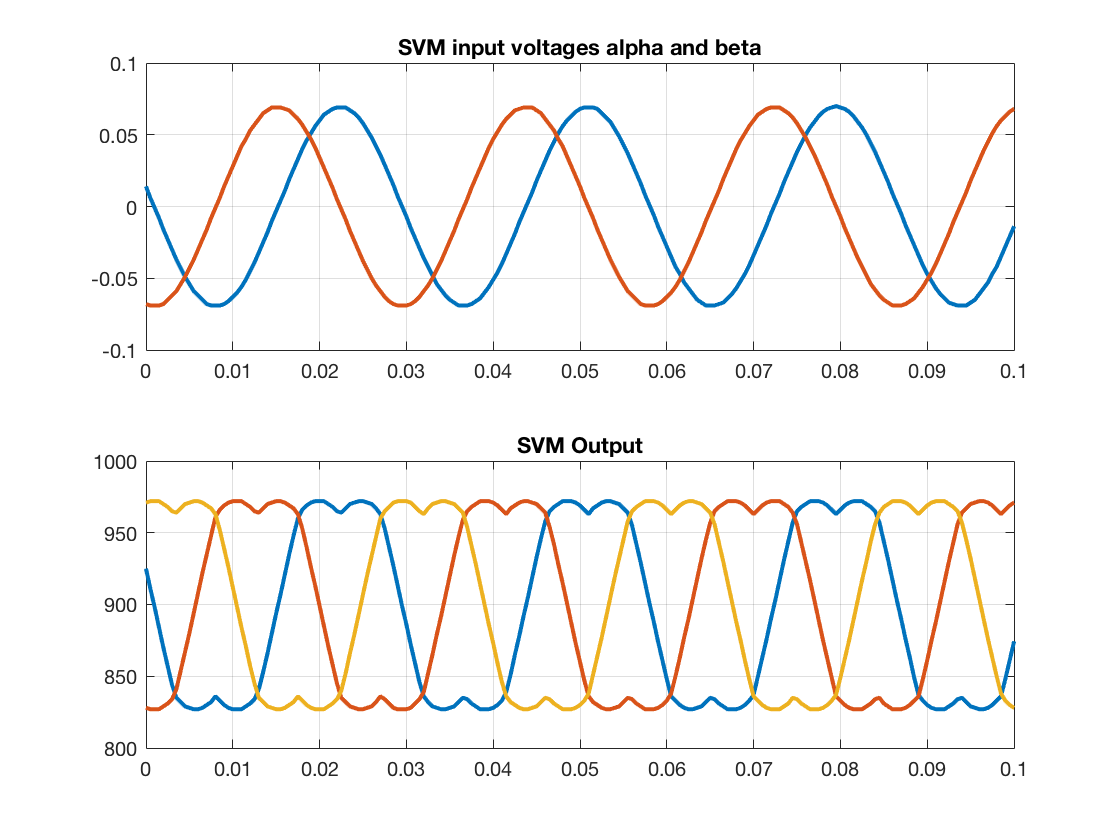
\includegraphics[width=0.8\linewidth]{images/valmcsvm.png}
	\caption{Validierung SVPWM Raumvektormodulation}
	\label{fig:svpwm}
\end{figure}

Im unteren Plot der Abbildung \ref{fig:svpwm} ist sehr gut der dreiphasige Sinus mit dritter harmonischer Welle zu sehen. Diese Werte entsprechen den Dutycyclen der MOSFETs.

\subsubsection*{Positions- und Geschwindigkeitsbeobachter} \label{val:obs}
Nun wird der Motor zwangskommutiert. Das heisst, dass wieder eine sinusförmige Spannung mit konstanter Frequenz und Amplitude berechnet und auf die H-Brücke geführt wird. Der Motor dreht nun mit einer konstanter Drehzahl. Die Ausgangswerte der Positions- und Geschwindigkeitsbeobachter werden erneut aufgezeichnet und mit dem Computer ausgewertet.

\begin{center}
	\begin{tabular}{l|c}
		\hline 
		$v_{d,set}$ & $0.0$ \\ \hline
		$v_{q,set}$ & $0.07$ \\ \hline
		$f_{set}$ & $35.0Hz$ \\ \hline
		Versorgungsspannung & $15V$ \\ \hline
	\end{tabular} 
	\captionof{table}{Messbedingungen Spannungsmessung Software}
	\label{tab:obsmessbed}
\end{center}

\begin{figure} [H]
	\centering
	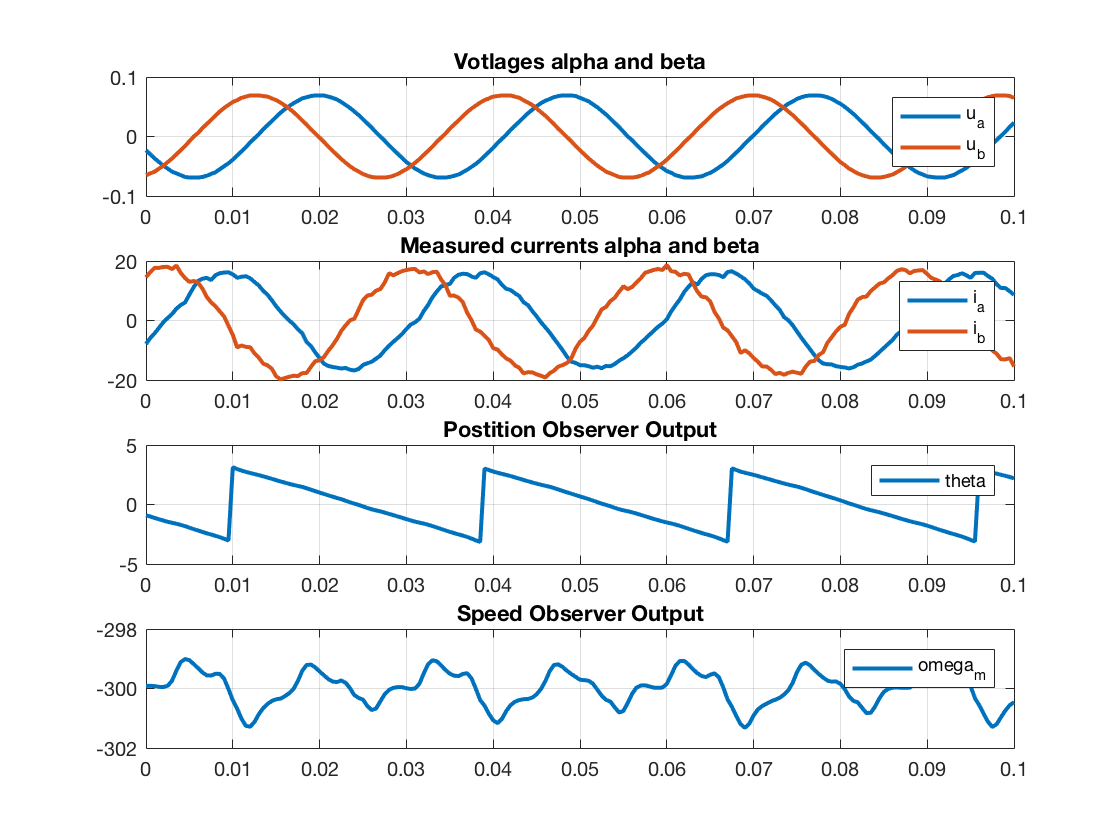
\includegraphics[width=0.8\linewidth]{images/valmcobserver.png}
	\caption{Validierung Positions- und Geschwindigkeitsbeobachter}
	\label{fig:observer}
\end{figure}

Abbildung \ref{fig:observer} zeigt in den ersten beiden Plots die Eingabewerte des Positionsbeobachters. Die gemessenen Ströme sind ungefiltert dargestellt und nur von kleinem Rauschen behaftet. Die Positionsschätzung theta hat ebenfalls nur einen kleinen Rippel und kann gut für die benötigten Transformationen verwendet werden.
Was in diesem Versuch nicht validier werden kann, ist der Phasenversatz zwischen wahrem und geschätztem Winkel. Dazu wären unter Anderem ein Drehgeber am Motor und eine Datenauswertung nötig, welche zeitkritisch die berechneten und gemessenen Grössen aufzeichnen kann.

Die Schätzung der Drehzahl schwingt um den Mittelwert von -300rpm was genau dem eingestellten Wert entspricht:

\begin{equation}
	\omega_m [rpm] = \frac{60 \cdot \omega_e}{p} = \frac{60 \cdot 35Hz}{7} = 300rpm
\end{equation}

Die Welligkeit wird vor dem Verwendung für den Stromregler tiefpassgefiltert.

\subsubsection*{D und Q Stromregler}
Der letzte Validierungsschritt für die Motorsteuerung auf dem Prüfstand ist die Überprüfung der D und Q Stromregler. Wie bei Validierungsschritt \ref{val:obs} werden die Daten der Regler auf dem Mikrocontroller zwischengespeichert und anschliessend auf dem Computer dargestellt. Bei dieser Validierung wird der Motor im Closed-Loop-Modus betrieben. Es wird softwaremässig ein Sollwertsprung ausgeführt.

\begin{center}
	\begin{tabular}{l|c}
		\hline 
		$i_{d,set}$ & $0$ \\ \hline
		$i_{q,set}$ & 3 auf 5 \\ \hline
		Versorgungsspannung & $21V$ \\ \hline
	\end{tabular} 
	\captionof{table}{Messbedingungen D und Q Stromregler}
	\label{tab:regmessbed}
\end{center}

\begin{figure} [H]
	\centering
	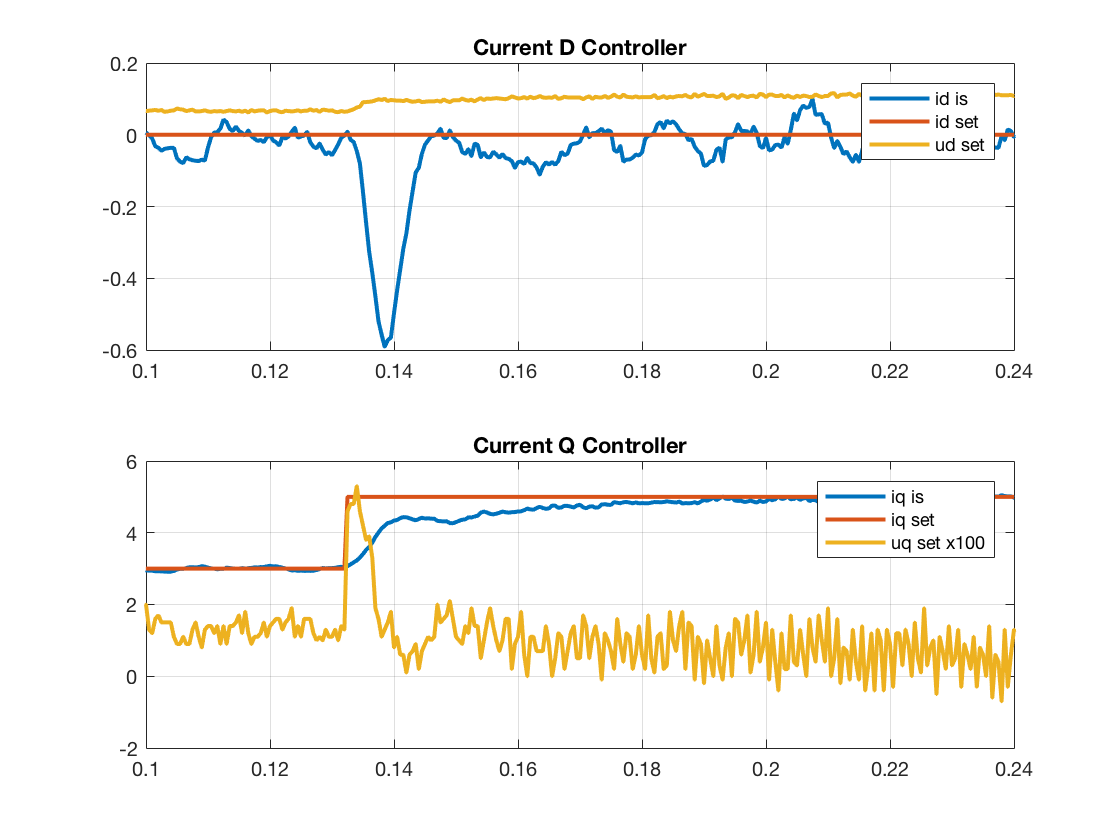
\includegraphics[width=0.8\linewidth]{images/valmccontrollers.png}
	\caption{Validierung D und Q Stromregler}
	\label{fig:reg}
\end{figure}

Abbildung \ref{fig:reg} zeigt die Sprungantwort der beiden Stromregler. Beide sind nicht perfekt und könnten noch optimiert werden. Da der Motor jedoch bei hohen Drehzahlen noch nicht dreht, wurde auf eine ausführliche Optimierung verzichtet. Was jedoch bestätigt werden kann ist, dass der Regler eine schnelle Sprungantwort hat und keine bleibende Regelabweichung dank I-Anteil vorhanden ist.


\subsubsection*{Fazit}
\todo{Anderer Titel?}
Die meisten Komponenten der Motorsteuerung funktionieren. Der Motor dreht jedoch nur bei langsamen Drehzahlen (kleiner 1000rpm) und mit wenig Drehmoment. Der Fehler liegt in der Implementierung des Stromreglers. Vermutlich ist es nur noch eine Sache der richtigen Parameter. Da das Umsetzen sehr zeitaufwändig ist, wurde darauf verzichtet.


%%%%%%%%%%%%%%%%%%%%%%%%%%%%%%%%%%%%%%%%%%%%%%%%%%%%%%%%%%%%%%%%
% Gesamtvalidierung
%%%%%%%%%%%%%%%%%%%%%%%%%%%%%%%%%%%%%%%%%%%%%%%%%%%%%%%%%%%%%%%%
\section{Gesamtvalidierung}
\label{ValidGesamtv}
Nach eingehendem Testen der einzelnen Komponenten wird das Gesamtprodukt getestet. Dabei wird primär die Lauffähigkeit des Longboards und die Zusammenarbeit der einzelnen Komponenten untereinander untersucht. Insbesondere werden die im Pflichtenheft festgelegten Kriterien überprüft. \\
\textbf{Steuerung:} Schaltet der Motor aus, wenn der Benutzer nicht mehr auf dem Longboard steht? Wie gross ist die maximale Distanz, über die die Funkübertragung noch funktioniert? \\
\textbf{Stromversorgung:} Funktioniert das aktive Balancing während dem Ladevorgang? Dazu werden die Zellspannungen während eines Ladevorganges überprüft und miteinander verglichen. Existiert der Überstromschutz?\\ \todo{gehört zur Stromvers-Valid! > gesamtvalid.frage??}
\textbf{Motoransteuerung:} Ist das Fahren des Longboards ohne aktivierter Antrieb möglich? \\
\\
Da das Longboard nicht fahrtüchtig ist, kann die Gesamtvalidierung nicht gemacht werden, deshalb sind keine Ergebnisse vorhanden.

\section{Alltagstauglichkeit}
\label{ValidAlltag}
Wie bereits angetönt, soll das fertige Board anhand von Testpersonen unterschiedlicher Skate-Erfahrung getestet werden. Die sanfte Anfahrmöglichkeit, die Manövrierfähigkeit und das allgemeine Wohlbefinden des Skaters sind die entscheidenden Kriterien. 
Testpersonen werden zufällig ausgewählt und die Bewertungen erfolgten nach subjektivem Einschätzen. 
Da das Longboard nicht fahrtüchtig ist, kann die Alltagstauglichkeit nicht getestet werden.
\todo{unterschiedliche Zeiten (soll getestet werden - wurden ausgewählt / bereits getestet)}

